%%% lorem.tex --- 
%% 
%% Filename: lorem.tex
%% Description: 
%% Author: Ola Leifler
%% Maintainer: 
%% Created: Wed Nov 10 09:59:23 2010 (CET)
%% Version: $Id$
%% Version: 
%% Last-Updated: Wed Nov 10 09:59:47 2010 (CET)
%%           By: Ola Leifler
%%     Update #: 2
%% URL: 
%% Keywords: 
%% Compatibility: 
%% 
%%%%%%%%%%%%%%%%%%%%%%%%%%%%%%%%%%%%%%%%%%%%%%%%%%%%%%%%%%%%%%%%%%%%%%
%% 
%%% Commentary: 
%% 
%% 
%% 
%%%%%%%%%%%%%%%%%%%%%%%%%%%%%%%%%%%%%%%%%%%%%%%%%%%%%%%%%%%%%%%%%%%%%%
%% 
%%% Change log:
%% 
%% 
%% RCS $Log$
%%%%%%%%%%%%%%%%%%%%%%%%%%%%%%%%%%%%%%%%%%%%%%%%%%%%%%%%%%%%%%%%%%%%%%
%% 
%%% Code:

\chapter{Resultat}
\label{cha:results}

Detta kapitel tar upp de resultat som projektgruppen kommit fram till under projektets gång.

\section{Systembeskrivning}

Projektgruppen definierade en tydlig design av applikationen innan implementationen påbörjades. Detta var för att försäkra sig om att applikationen skulle bli av hög kvalitet och eventuella designproblem skulle hittas tidigt i projektet.

\subsection{Systemanatomi}
\label{beskrivning-systemanatomi}
Under iteration ett producerade projektgruppen en systemanatomi av applikationen som skulle utveckas. Denna producerades utifrån de use-cases och krav kunden hade tillhandahållit. I figur \ref{fig:systemanatomi_graf} visas systemanatomin för hela systemet och i \ref{fig:systemanatomi_spel} visas den för själva spelet.

\begin{figure}[H]
    \centering
    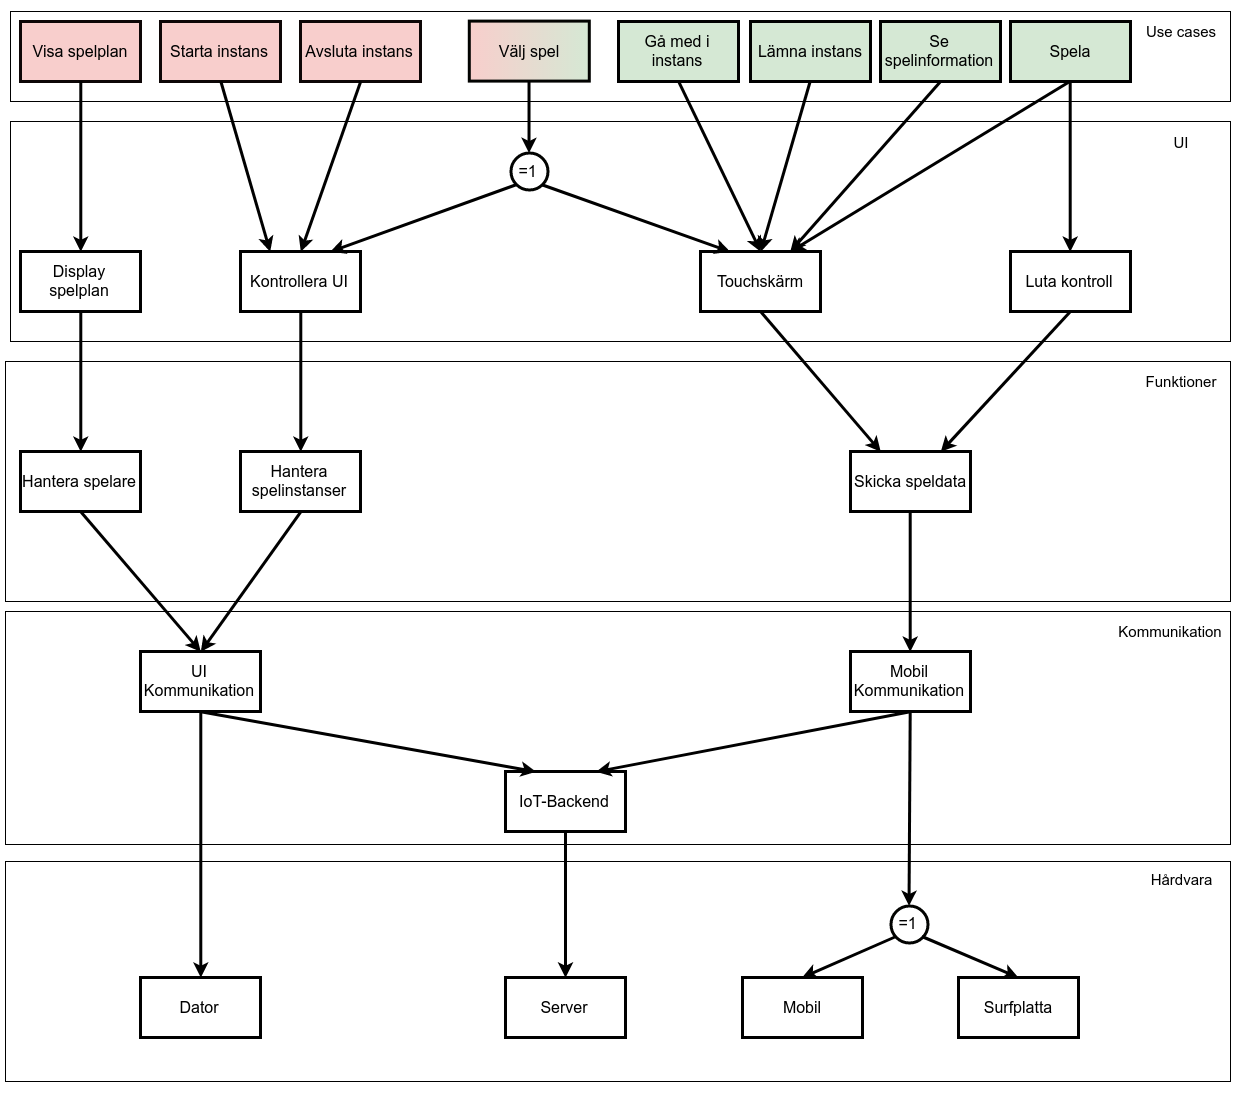
\includegraphics[scale=0.3]{systemanatomi_graf}
    \caption{Överblick av systemanatomin}
    \label{fig:systemanatomi_graf}
\end{figure}

\begin{figure}[H]
    \centering
    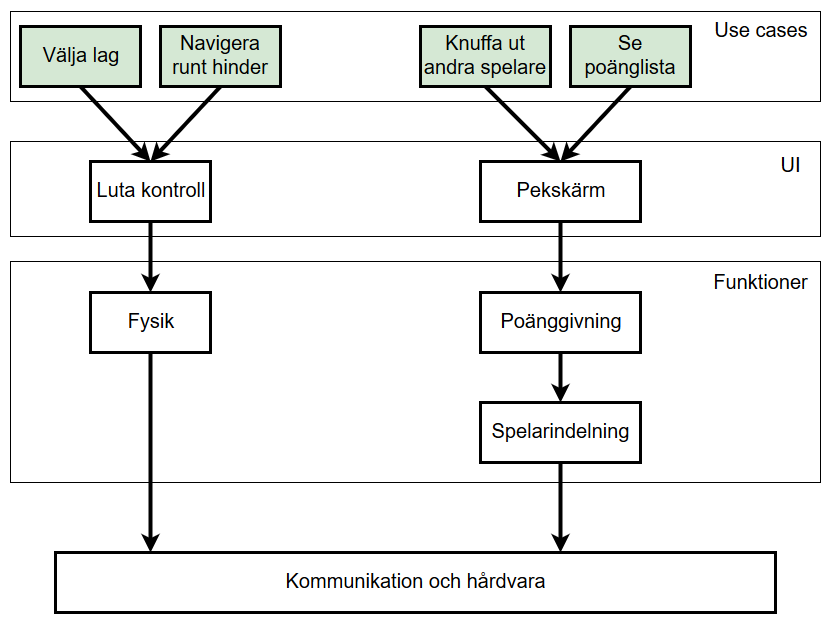
\includegraphics[scale=0.3]{systemanatomi_spel}
    \caption{Överblick av systemanatomin för spelet}
    \label{fig:systemanatomi_spel}
\end{figure}


\pagebreak

\subsection{Moduler}
Projektgruppen använde sig av den generella strukturen av systemet, kundens krav och systemanatomin för att skapa en mer detaljerad arkitektur. I figur \ref{fig:konceptarkitektur} kan man se den övergripande strukturen av modulerna som finns i applikationen.

\begin{figure}[h]
    \centering
    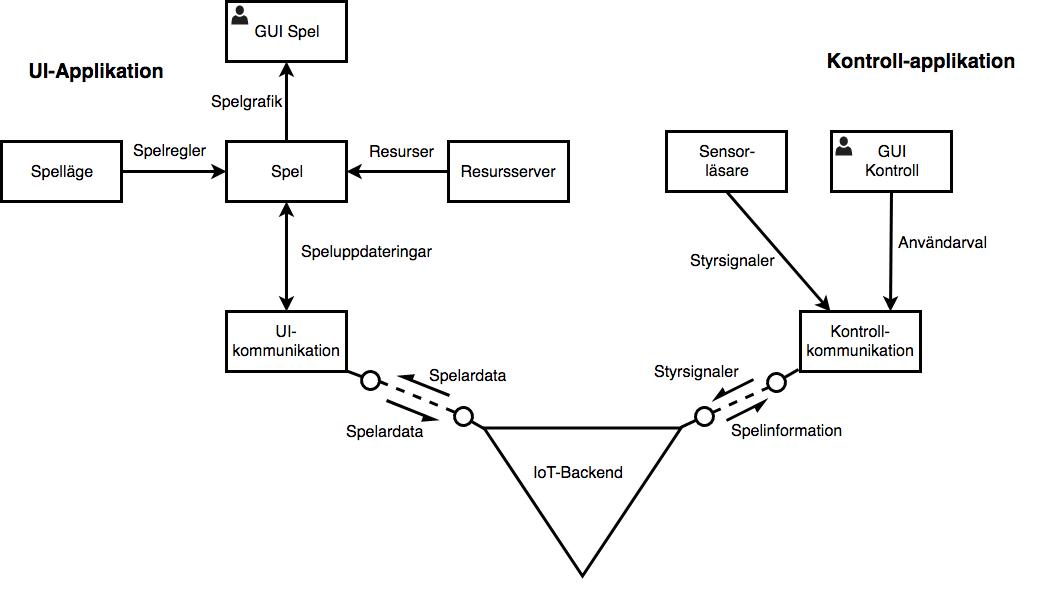
\includegraphics[scale=0.3]{konceptarkitektur}
    \caption{Överblick av systemets moduler}
    \label{fig:konceptarkitektur}
\end{figure}

\pagebreak


\subsubsection*{Ansvarsområden}
Varje modul i systemet har ett eget ansvarsområde. Nedan följer en förtydling på vad varje modul ansvarar för.

\begin{labeling}{\small{\textbf{Kontrollkommunikation}}}
    \item [\small{\textbf{GUI Spel}}]
        \begin{itemize}
            \item Visa upp spelplanen
            \item Visa upp menyer
            \item Starta spel med specifika inställningar
            \newline
        \end{itemize}

    \item [\small{\textbf{Spelläge}}]
        \begin{itemize}
            \item Sätta upp regler för spelet
            \item Avgöra vilka resurser spelet ska innehålla
            \item Avgöra vad som ska ske vid olika tillfällen i spelet
            \newline
        \end{itemize}

    \item [\small{\textbf{Spel}}]
        \begin{itemize}
            \item Hålla koll på de olika spelarna
            \item Tillhandahålla grundläggande spelmekanik
            \newline
        \end{itemize}

    \item [\small{\textbf{Resursserver}}]
        \begin{itemize}
            \item Lagra vilka resurser som finns
            \item Ladda in resurser
            \newline
        \end{itemize}

    \item [\small{\textbf{UI-kommunikation}}]
        \begin{itemize}
            \item Upprätta uppkoppling mot server
            \item Förpacka data för kommunikation
            \newline
        \end{itemize}

    \item [\small{\textbf{Sensorläsare}}]
        \begin{itemize}
            \item Läsa av data från sensor
            \item Abstrahera sensordata till standardiserad form
            \item Konfigurera sensor
            \newline
        \end{itemize}

    \item [\small{\textbf{GUI-kontroll}}]
        \begin{itemize}
            \item Visa menyer för att gå med i spelinstans
            \item Visa spelinformation om det pågående spelet
            \item Tillhandahålla knappar på skärmen
            \newline
        \end{itemize}

    \item [\small{\textbf{Kontrollkommunikation}}]
        \begin{itemize}
            \item Upprätta uppkoppling mot server
            \item Förpacka data för kommunikation
            \newline
        \end{itemize}

    \item [\small{\textbf{IoT-Backend}}]
        \begin{itemize}
            \item Dirigera data mellan olika Kontroll-applikationer och olika instanser av UI-applikationen
            \item Verifiera koder för att gå med i specifika spelinstanser
            \newline
        \end{itemize}
\end{labeling}


\section{Gemensamma erfarenheter}
Denna del tar upp diverse erfarenheter projektgruppen råkat ut för, både innan och under projektets gång.

\subsection{Erfarenheter av systemanatomi}
Systemanatomin som presenterades under \ref{beskrivning-systemanatomi} användes för att ge en enhetlig ochn helteckande bild över hur det färdiga systemet skulle se ut. Dock var arbetet med att ta fram själva systemanatomin är något som tog relativt lång tid, om den värderas mot den nytta gruppen haft av den. Den blev mer ett verktyg som gruppen kunde använda för att verifiera resterande arkitekturbeskrivningar. Gruppen känner att själva processen att att producera anatomin var nyttigare än den resulterande bilden, då det skapade en öppen dialog om systemets helhet.

\subsection{Tidigare erfarenheter}
Alla av projektets medlemmar hade studerat mer än två år på respektive program innan detta projekt startades. På grund hade alla haft möjligheten att medverka i några större projekt och var därför ganska vana vid hur arbetet gick till. Dock var det få som hade erfarenhet med webbutveckling och spelprogrammering, något som hade stort fokus i detta projekt. Detta var dock inget större problem då de mer erfarna kunde hjälpa resten att komma igång.

\subsection{Nya erfarenheter}
Under projeketets gång har alla medlemmar fått använda sig av nya verktyg och metoder som de inte haft tidigare erfarenhet av. De projektmedlemmar som tidigare saknade erfarenhet inom webbutveckling och spelprogrammering har fått chansen att sätta sig in i dessa. För att förbättra denna process hjälpte de som redan var erfarana inom ämnet till med att svara på frågor och komma med tips och idéer. Under projekts gång tillkom en del nya paket och ramverk. Ett exempel på detta PIXI.JS, ramverket UI-applikationen använder för att rita ut spelet. Det var ingen i projektgruppen som hade jobbat med detta ramverk innan, så några i gruppen fick tillsammans sätta sig in i hur det fungerade och utbilda resterande vid behov. Detta gällde även en del av det olika NPM-paketen som installerades och användes i projeket.


\subsection{Tidsbrist}
I början av projektet hade gruppen bra tidsplanering och lämnade in första iterationen i god tid för att sedan ta det lugnt. I början av iteration två satsade gruppen i huvudsak på utveckling och lämnade dokumentskrivning till senare, vilket visade sig vara en missbedömning. Detta ledde till att det blev stressigt framåt slutet av iteration två vilket kan ha påverkat dokumentkvaliteten negativt. Gruppen noterade dock detta och tog upp på kommande gruppmöten hur de skulle kunna göra det bättre inför kommande iterationer. Nästa iteration delades upp i en tydligare utvecklingsfas och dokumentfas, vilket tillät en bättre planering och fördelning av tiden. 

\subsection{Tekniska erfarenheter}
Projektgruppen utvecklade applikationen i ramverket React som har något som kallas för states. Projektgruppen märkte att det snabbt kunde bli något rörigt när man introducerade flera lager av komponenter. Detta problem löser andra webbapplikationer genom extra verktyg för state-hantering, och gruppen reflekterade över dessa men besluta emot att använda något liknande. Det visade sig dock i senare delen av projektet att hanteringen av states blev något rörig, då gruppen använt sig av fler komponenter än vad som först uppskattats. Detta ledde till att implementationen av nya komponenter som hamnade mellan redan existerande komponenter blev något jobbig. Detta berodde främst på att data som tidigare skickats från komponent \texttt{A} till \texttt{B} nu behövde skickas från \texttt{A} till \texttt{C} och sen från \texttt{C} till \texttt{B}, när man introducerade den ny komponenten \texttt{C} mellan \texttt{A} och \texttt{B}. Detta ledde till att all data som tidigare skickades mellan \texttt{A} och \texttt{B} nu också behövde skickas till \texttt{C}, trots att den kunde vara data \texttt{C} inte använde sig av. I grafik överblick kan ses i figur \ref{fig:middle_component}

\begin{figure}[H]
    \centering
    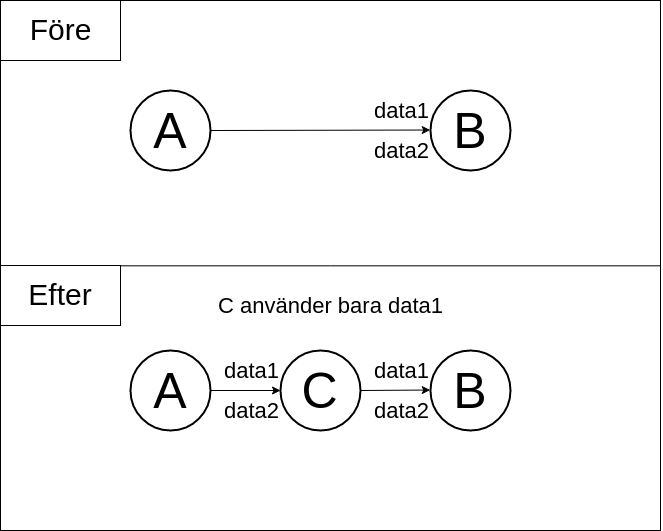
\includegraphics[scale=0.3]{middle_component}
    \caption{Överblick hur implementation av mittenkomponent kan ge ett ineffektivt dataflöde}
    \label{fig:middle_component}
\end{figure}



%%%%%%%%%%%%%%%%%%%%%%%%%%%%%%%%%%%%%%%%%%%%%%%%%%%%%%%%%%%%%%%%%%%%%%
%%% lorem.tex ends here

%%% Local Variables: 
%%% mode: latex
%%% TeX-master: "demothesis"
%%% End: 
